\setlength{\headheight}{14.49998pt}
\titleformat{\section}
  {\normalfont\LARGE\bfseries\centering}
  {\thesection}{1em}{}  


\vspace{0.2cm}{\color{gray}\hrule}
\section{Theorie}


\subsection{Werking van een PID-regelaar}

Een PID-regelaar (Proportioneel-Integrerend-Differentiërend) is een veelgebruikte terugkoppelingsregelaar in de regeltechniek, die als doel heeft een systeem naar een gewenste waarde (setpoint) te sturen door continu het verschil (de fout) tussen die gewenste waarde en de gemeten systeemoutput te corrigeren.
De PID-regelaar bestaat uit drie componenten:
\begin{itemize}
  \item \textbf{Proportioneel (P):} Deze component reageert op de huidige fout. Hoe groter de fout, hoe sterker de aansturing. Dit zorgt voor een directe correctie, maar kan leiden tot een blijvende fout (steady-state error) als deze component alleen wordt gebruikt.
  \item \textbf{Integrerend (I):} Deze component reageert op de opgetelde (geïntegreerde) fout in de tijd. Hierdoor kan de regelaar kleine resterende fouten wegwerken en wordt het systeem naar het exacte setpoint geduwd. Te veel integratie kan echter leiden tot traagheid of instabiliteit.
  \item \textbf{Differentiërend (D):} Deze component reageert op de snelheid waarmee de fout verandert. Dit helpt om snelle veranderingen te dempen en voorkomt overshoot door het systeem te vertragen voordat het het setpoint bereikt. De D-term maakt het systeem reactiever en stabieler bij plotselinge veranderingen.
\end{itemize}
De regeloutput \( u(t) \) van een PID-regelaar wordt meestal als volgt beschreven:
\begin{equation}
u(t) = K_p \cdot e(t) + K_i \cdot \int_0^t e(\tau)\,d\tau + K_d \cdot \frac{de(t)}{dt}
\label{eq:pid}
\end{equation}
waarbij:
\[
\begin{aligned}
e(t) &= r(t) - y(t) \quad \text{(de fout tussen de referentie en gemeten waarde)} \\
K_p  &= \text{proportionele versterkingsfactor} \\
K_i  &= \text{integrerende versterkingsfactor} \\
K_d  &= \text{differentiërende versterkingsfactor}
\end{aligned}
\]
Een goed afgestemde PID-regelaar zorgt voor een snelle respons, minimale overshoot en een stabiele benadering van het setpoint zonder blijvende fout. Hoewel we in dit onderzoek niet in detail ingaan op de afstemming van PID-parameters, is het belangrijk te vermelden dat dit een cruciaal onderdeel is van het gebruik van PID-regelaars in de praktijk. De afstemming wordt meestal handmatig gedaan en dit is meestal een iteratief proces waarbij de waarden van \(K_p\), \(K_i\) en \(K_d\) worden aangepast op basis van de prestaties van het systeem. Er zijn verschillende methoden voor PID-afstemming, zoals de Ziegler-Nichols-methode, maar deze vallen buiten de scope van dit onderzoek. In dit onderzoek richten we ons op het vervangen van de PID-regelaar door een neuraal netwerk, waarbij we de nadruk leggen op hrt gedrag van de PID regelaar en de mogelijkheid om dit gedrag te repliceren met een neuraal netwerk.
\subsection{Neurale netwerken - basisprincipes}
Een neuraal netwerk is een wiskundig model dat is geïnspireerd op de werking van het menselijk brein. Het bestaat uit een verzameling onderling verbonden knopen, ook wel neuronen genoemd, die georganiseerd zijn in lagen: een inputlaag, één of meerdere verborgen lagen en een outputlaag. Elke verbinding tussen neuronen heeft een gewicht dat bepaalt hoe sterk een input wordt doorgegeven. Tijdens het doorlopen van het netwerk wordt elke input vermenigvuldigd met het bijbehorende gewicht, opgeteld met een bias en vervolgens door een activatiefunctie gehaald. Deze activatiefunctie bepaalt of en in welke mate het neuron wordt geactiveerd. Het leerproces van een neuraal netwerk gebeurt aan de hand van trainingsdata. Op basis van de fout tussen de voorspelde output en de werkelijke waarde worden de gewichten aangepast met behulp van een algoritme zoals bijvoorbeeld backpropagation in combinatie met gradient descent. Door herhaaldelijk trainen op veel voorbeelden leert het netwerk patronen en relaties herkennen in de data. Neurale netwerken zijn bijzonder krachtig in het modelleren van complexe, niet-lineaire systemen, en worden daarom veel gebruikt in toepassingen zoals beeldherkenning, spraakherkenning en regeltechniek.
\begin{center}
\centering
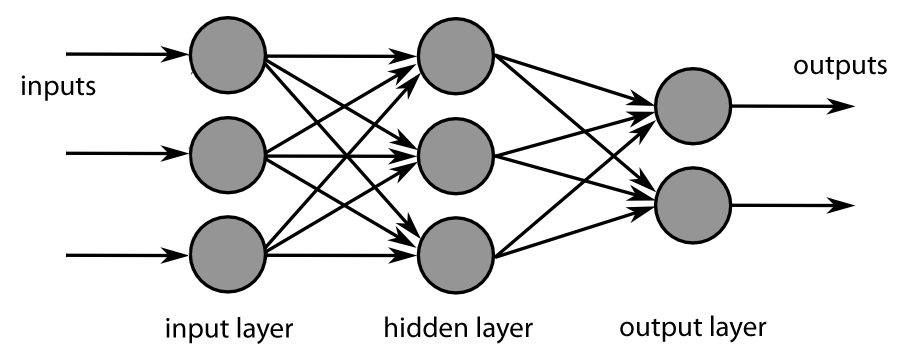
\includegraphics[width=0.45\textwidth]{./afbeeldingen/Neuraalnetwerkpng.png}
\label{fig:Illustratie_neuraal_netwerk}
\captionof{figure}{Illustratie van een neuraal netwerk}
\end{center}
\subsection{vergelijking PID versus NN-regelaars}
Zowel PID-regelaars als neurale netwerken kunnen worden ingezet om systemen te regelen, maar hun werking, toepassingsgebied en eigenschappen verschillen sterk.
\subsubsection{Verschillen}
\begin{itemize}
  \item \textbf{Regelprincipe:} Een PID-regelaar is gebaseerd op een vaste wiskundige formule die werkt met de fout tussen gewenste en gemeten waarden. Een neuraal netwerk leert juist op basis van voorbeelddata een model van het systeemgedrag.
  \item \textbf{Aanpasbaarheid:} PID-regelaars hebben vaste parameters \(K_p\), \(K_i\), \(K_d\) die handmatig of via tuning bepaald worden. Neurale netwerken leren automatisch complexe relaties tijdens het trainen, zonder expliciet geprogrammeerde regels. 
  \item \textbf{Complexiteit:} PID-regelaars zijn relatief eenvoudig te implementeren en begrijpen. Neurale netwerken zijn complexer en vereisen meer rekenkracht en data.
  \item \textbf{Flexibiliteit:} PID is minder geschikt voor sterk niet-lineaire systemen of systemen met veel vertraging. Neurale netwerken kunnen deze situaties beter aan, mits voldoende training.
  \item \textbf{Transparantie:} PID-regelaars zijn goed uitlegbaar. Neurale netwerken zijn vaak 'black boxes', waarbij het moeilijk is om te achterhalen waarom een bepaalde beslissing wordt genomen.
\end{itemize}
\subsubsection{Overeenkomsten}
\begin{itemize}
  \item Beide regelmethoden kunnen gebruikt worden voor het aansturen van dynamische systemen.
  \item Beide maken gebruik van foutsignalen (in neurale netwerken impliciet tijdens het trainen).
  \item Beide kunnen met feedback werken om de systeemoutput te corrigeren.
  \item Beide vereisen afstemming of training om goed te presteren in een specifieke toepassing.
\end{itemize}
In veel gevallen kan een neuraal netwerk zelfs worden getraind om het gedrag van een PID-regelaar na te bootsen, wat de basis vormt voor het vervangen of verbeteren van klassieke regelsystemen met AI-gebaseerde methoden.
\subsection{keuze van netwerkarchitecturen }
Bij het kiezen van een netwerkarchitectuur voor het vervangen van een PID-regelaar door een neuraal netwerk, zijn er verschillende opties beschikbaar, afhankelijk van de aard van het systeem en de beschikbare data. Twee veelgebruikte architecturen zijn feedforward netwerken en recurrente netwerken. Ik heb hierbij gekeken naar de volgende aspecten:
\begin{itemize}
  \item \textbf{Feedforward netwerken:} Deze netwerken zijn geschikt voor statische mapping van invoer naar uitvoer, waarbij de informatie slechts in één richting stroomt. Ze zijn eenvoudig te implementeren en kunnen goed presteren bij systemen met relatief eenvoudige dynamiek. Ze zijn echter minder geschikt voor systemen met tijdsafhankelijke gedragspatronen.      
  \item \textbf{Recurrente netwerken (RNN):} Deze netwerken zijn ontworpen om tijdsafhankelijke data te verwerken door informatie van eerdere tijdstappen te onthouden. Ze zijn nuttig voor systemen waarbij de huidige output afhankelijk is van eerdere inputs, zoals bij dynamische systemen. RNN's kunnen echter complexer zijn om te trainen en vereisen meer rekenkracht.
  \item   \textbf{Convolutionele netwerken (CNN):} Hoewel CNN's voornamelijk worden gebruikt voor beeldverwerking, kunnen ze ook nuttig zijn voor systemen met ruimtelijke of temporele patronen. Ze zijn minder gebruikelijk voor regeltoepassingen, maar kunnen nuttig zijn als het systeem complexe patronen vertoont.
  \item \textbf{Long Short-Term Memory (LSTM):} Dit is een type RNN dat speciaal is ontworpen om lange-termijn afhankelijkheden te onthouden. LSTM's zijn zeer geschikt voor systemen met complexe dynamiek en tijdsafhankelijke gedragspatronen, maar ze zijn ook complexer en vereisen meer data om goed te presteren.
  \item   \textbf{Transformer netwerken:} Deze netwerken zijn ontworpen voor het verwerken van sequentiële data en zijn zeer effectief gebleken in natuurlijke taalverwerking. Ze kunnen ook worden toegepast op regeltoepassingen, vooral wanneer er veel tijdsafhankelijke data beschikbaar is. Ze zijn echter complex en vereisen aanzienlijke rekenkracht.
\end{itemize}
De keuze van de netwerkarchitectuur hangt af van de specifieke kenmerken van het systeem, de beschikbare data en de vereiste prestaties. Voor eenvoudige systemen kan een feedforward netwerk voldoende zijn, terwijl voor complexere systemen met tijdsafhankelijke gedragspatronen een RNN of LSTM meer geschikt kan zijn. Het is belangrijk om de architectuur te kiezen die het beste past bij de aard van het systeem en de doelstellingen van de regeling.
\subsection{Vergelijking van prestaties}
De prestaties van een neuraal netwerk in vergelijking met een PID-regelaar kunnen op verschillende manieren worden beoordeeld, afhankelijk van de specifieke toepassing en de doelstellingen van de regeling. Enkele belangrijke prestatie-indicatoren zijn:
\begin{itemize}
  \item \textbf{Nauwkeurigheid:} Hoe goed het neuraal netwerk de gewenste output kan voorspellen in vergelijking met de PID-regelaar. Dit kan worden gemeten aan de hand van de fout tussen de voorspelde en werkelijke waarden.
  \item \textbf{Stabiliteit:} Hoe stabiel het systeem is bij het bereiken van de gewenste output. Een PID-regelaar kan soms oscillaties vertonen, terwijl een goed getraind neuraal netwerk deze kan verminderen of elimineren.
  \item \textbf{Snelheid:} Hoe snel het neuraal netwerk kan reageren op veranderingen in de input. Dit is vooral belangrijk in real-time toepassingen waar snelle aanpassingen nodig zijn.
  \item \textbf{Robuustheid:} Hoe goed het neuraal netwerk presteert onder verschillende omstandigheden, zoals verstoringen of veranderingen in de systeemparameters. Een PID-regelaar kan soms gevoelig zijn voor veranderingen in de omgeving, terwijl een neuraal netwerk mogelijk beter kan generaliseren.
  \item \textbf{Complexiteit:} Hoe complex het neuraal netwerk is in vergelijking met de PID-regelaar. Een PID-regelaar is relatief eenvoudig te implementeren en te begrijpen, terwijl een neuraal netwerk meer rekenkracht en data vereist.
  \item \textbf{Trainings- en implementatietijd:} Hoe lang het duurt om het neuraal netwerk te trainen en te implementeren in vergelijking met de PID-regelaar. Een PID-regelaar kan snel worden ingesteld, terwijl een neuraal netwerk mogelijk meer tijd nodig heeft voor training en afstemming.
\end{itemize}
De vergelijking van prestaties tussen een neuraal netwerk en een PID-regelaar hangt af van de specifieke toepassing en de doelstellingen van de regeling. In sommige gevallen kan een neuraal netwerk betere prestaties leveren, terwijl in andere gevallen een PID-regelaar voldoende kan zijn. Het is belangrijk om de juiste prestatie-indicatoren te kiezen en de resultaten zorgvuldig te analyseren om een weloverwogen beslissing te nemen.
\subsection{Implementatie op embedded systemen}
De implementatie van een neuraal netwerk op embedded systemen, zoals microcontrollers of FPGA's, brengt specifieke uitdagingen en overwegingen met zich mee. Deze systemen hebben vaak beperkte rekenkracht, geheugen en energieverbruik in vergelijking met traditionele computers. Daarom is het belangrijk om de volgende aspecten in overweging te nemen bij de implementatie van een neuraal netwerk op embedded systemen:
\begin{itemize}
  \item \textbf{Modeloptimalisatie:} Het neuraal netwerk moet worden geoptimaliseerd voor de beperkte rekenkracht en geheugen van het embedded systeem. Dit kan onder meer het verminderen van het aantal parameters, het gebruik van quantisatie of het toepassen van modelcompressie omvatten.
  \item \textbf{Efficiënte inferentie:} De inferentie (voorspellingsfase) van het neuraal netwerk moet efficiënt worden uitgevoerd. Dit kan worden bereikt door gebruik te maken van speciale hardwareversnellers, zoals Tensor Processing Units (TPU's) of Field Programmable Gate Arrays (FPGA's), die zijn ontworpen voor het uitvoeren van neurale netwerken.
  \item \textbf{Real-time prestaties:} Het neuraal netwerk moet in staat zijn om real-time voorspellingen te doen, wat betekent dat de inferentietijd snel genoeg moet zijn om te voldoen aan de vereisten van de toepassing. Dit kan worden bereikt door het netwerk te optimaliseren voor snelheid en door gebruik te maken van efficiënte algoritmen.
  \item \textbf{Compatibiliteit met hardware:} Het neuraal netwerk moet compatibel zijn met de specifieke hardware van het embedded systeem. Dit kan onder meer het gebruik van specifieke bibliotheken of frameworks omvatten die zijn geoptimaliseerd voor de gekozen hardware.
  \item \textbf{Ondersteuning voor machine learning frameworks:} Het is belangrijk om te kiezen voor machine learning frameworks die ondersteuning bieden voor embedded systemen, zoals TensorFlow Lite, Keras of PyTorch Mobile. Deze frameworks zijn ontworpen om neurale netwerken te optimaliseren en te implementeren op beperkte hardware.
\end{itemize}
Door rekening te houden met deze aspecten kan een neuraal netwerk effectief worden geïmplementeerd op embedded systemen, waardoor het mogelijk wordt om de voordelen van machine learning te benutten in toepassingen met beperkte middelen. Dit opent de deur naar nieuwe mogelijkheden voor automatisering, controle en optimalisatie in diverse industrieën en toepassingen.

